\chapter{OsmocomBB}
\section{Installation}
\label{sec:osmo_install}
The environment used for this project was a Thinkpad X220 Tablet running Xubuntu Linux 11.10.
The instructions should work for any other distribution of the Ubuntu product palette.

\begin{enumerate}
	\item Build libraries must be installed on the operating system to enable compiling libraries.
	\begin{lstlisting}
sudo apt-get install libtool shtool autoconf git-core 
pkg-config make gcc wget
	\end{lstlisting}
	\item The GNU Arm cross compiler toolchain needs to be installed so the firmware for the Motorola C123 can be built.
	It will be added as a repository to \texttt{sources} so it can be easily removed if it is not required any more.
	\begin{lstlisting}
sudo add-apt-repository ppa:bdrung/bsprak
sudo apt-get update
sudo apt-get install arm-elf-toolchain
	\end{lstlisting}
	\item The source code needs to be obtained.
	This can be either done by checking out the latest version of the framework from the developers, or by using the code on the CD.
	\begin{lstlisting}
git clone git://git.osmocom.org/osmocom-bb.git
	\end{lstlisting}
	\item At this point some firmwares had build errors, therefore we will compile only the firmware for the Calypso board used by the Motorola C123.
	This constraint might not be necessary if a newer version of the framework is used.
	In the \texttt{src} directory of the OsmocomBB framework the build process can be started.
	\begin{lstlisting}
make BOARDS=compal_e88
	\end{lstlisting}
	\item If a new version of OsmocomBB is used, the extra code from this project must be included in the build.
	The two files \texttt{catcher.c} and \texttt{app\_catcher.c} must be moved to \texttt{osmocom-bb/src/host/layer23/src/misc} and the \texttt{Makefile.am} must be edited to include the new code.
	\begin{lstlisting}
bin_PROGRAMS = bcch_scan ... cbch_sniff catcher
catcher_SOURCES = ../common/main.c app_catcher.c
	\end{lstlisting}
\end{enumerate}

\section{Usage}
\label{sec:osmo_usage}
To use a program written in the framework, the Motorola C123 needs to be flashed with the custom firmware.
This can be done with the \texttt{osmocon} application. 
\begin{lstlisting}
cd src/host/osmocon
sudo ./osmocon -p /dev/ttyUSB0 -m c123xor
 ../../target/firmware/board/compal_e88/layer1.compalram.bin
\end{lstlisting}
After \texttt{osmocon} is started and running any application can be started with root privileges.
\begin{lstlisting}
cd ../layer23/src/misc/
sudo catcher
\end{lstlisting}

\section{Serial Cable Schematics}
\label{sec:osmo_serial_schematics}
A T191 unlock cable used to connect the Motorola C123 can either be obtained by ordering it from one of the mentioned stores or by building it from scratch.
The schematics can be seen in Figure \ref{fig:schematics}.

\begin{figure}
\centering
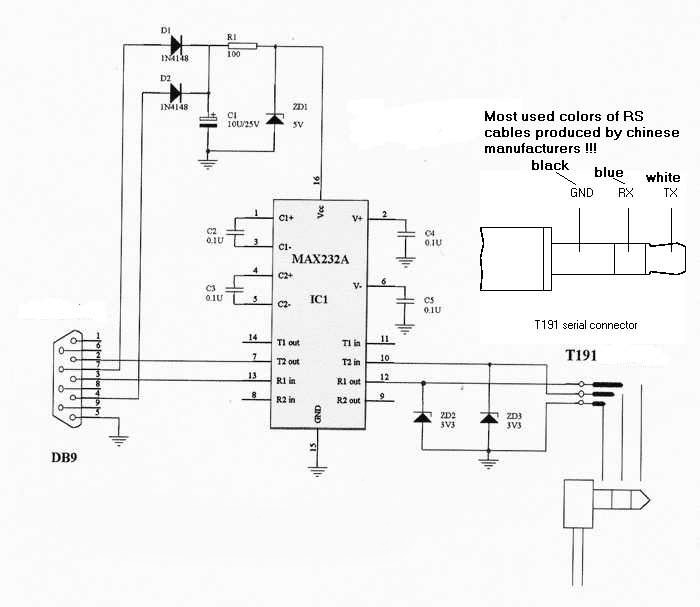
\includegraphics[width=.9\textwidth]{../Images/t191cable}
\caption{Schematics for the T191 unlock cable.}
\label{fig:schematics}
\end{figure}

\chapter{IMSI Catcher Detection System}
\section{Extextions}
\label{sec:extensions}
\section{Example Configuration}
\label{sec:example_config}
\chapter{System Information}
\label{sec:system_infos}
The following pages contain parsed System Information Messages of type 1-4  for reference.

\begin{figure}
\centering
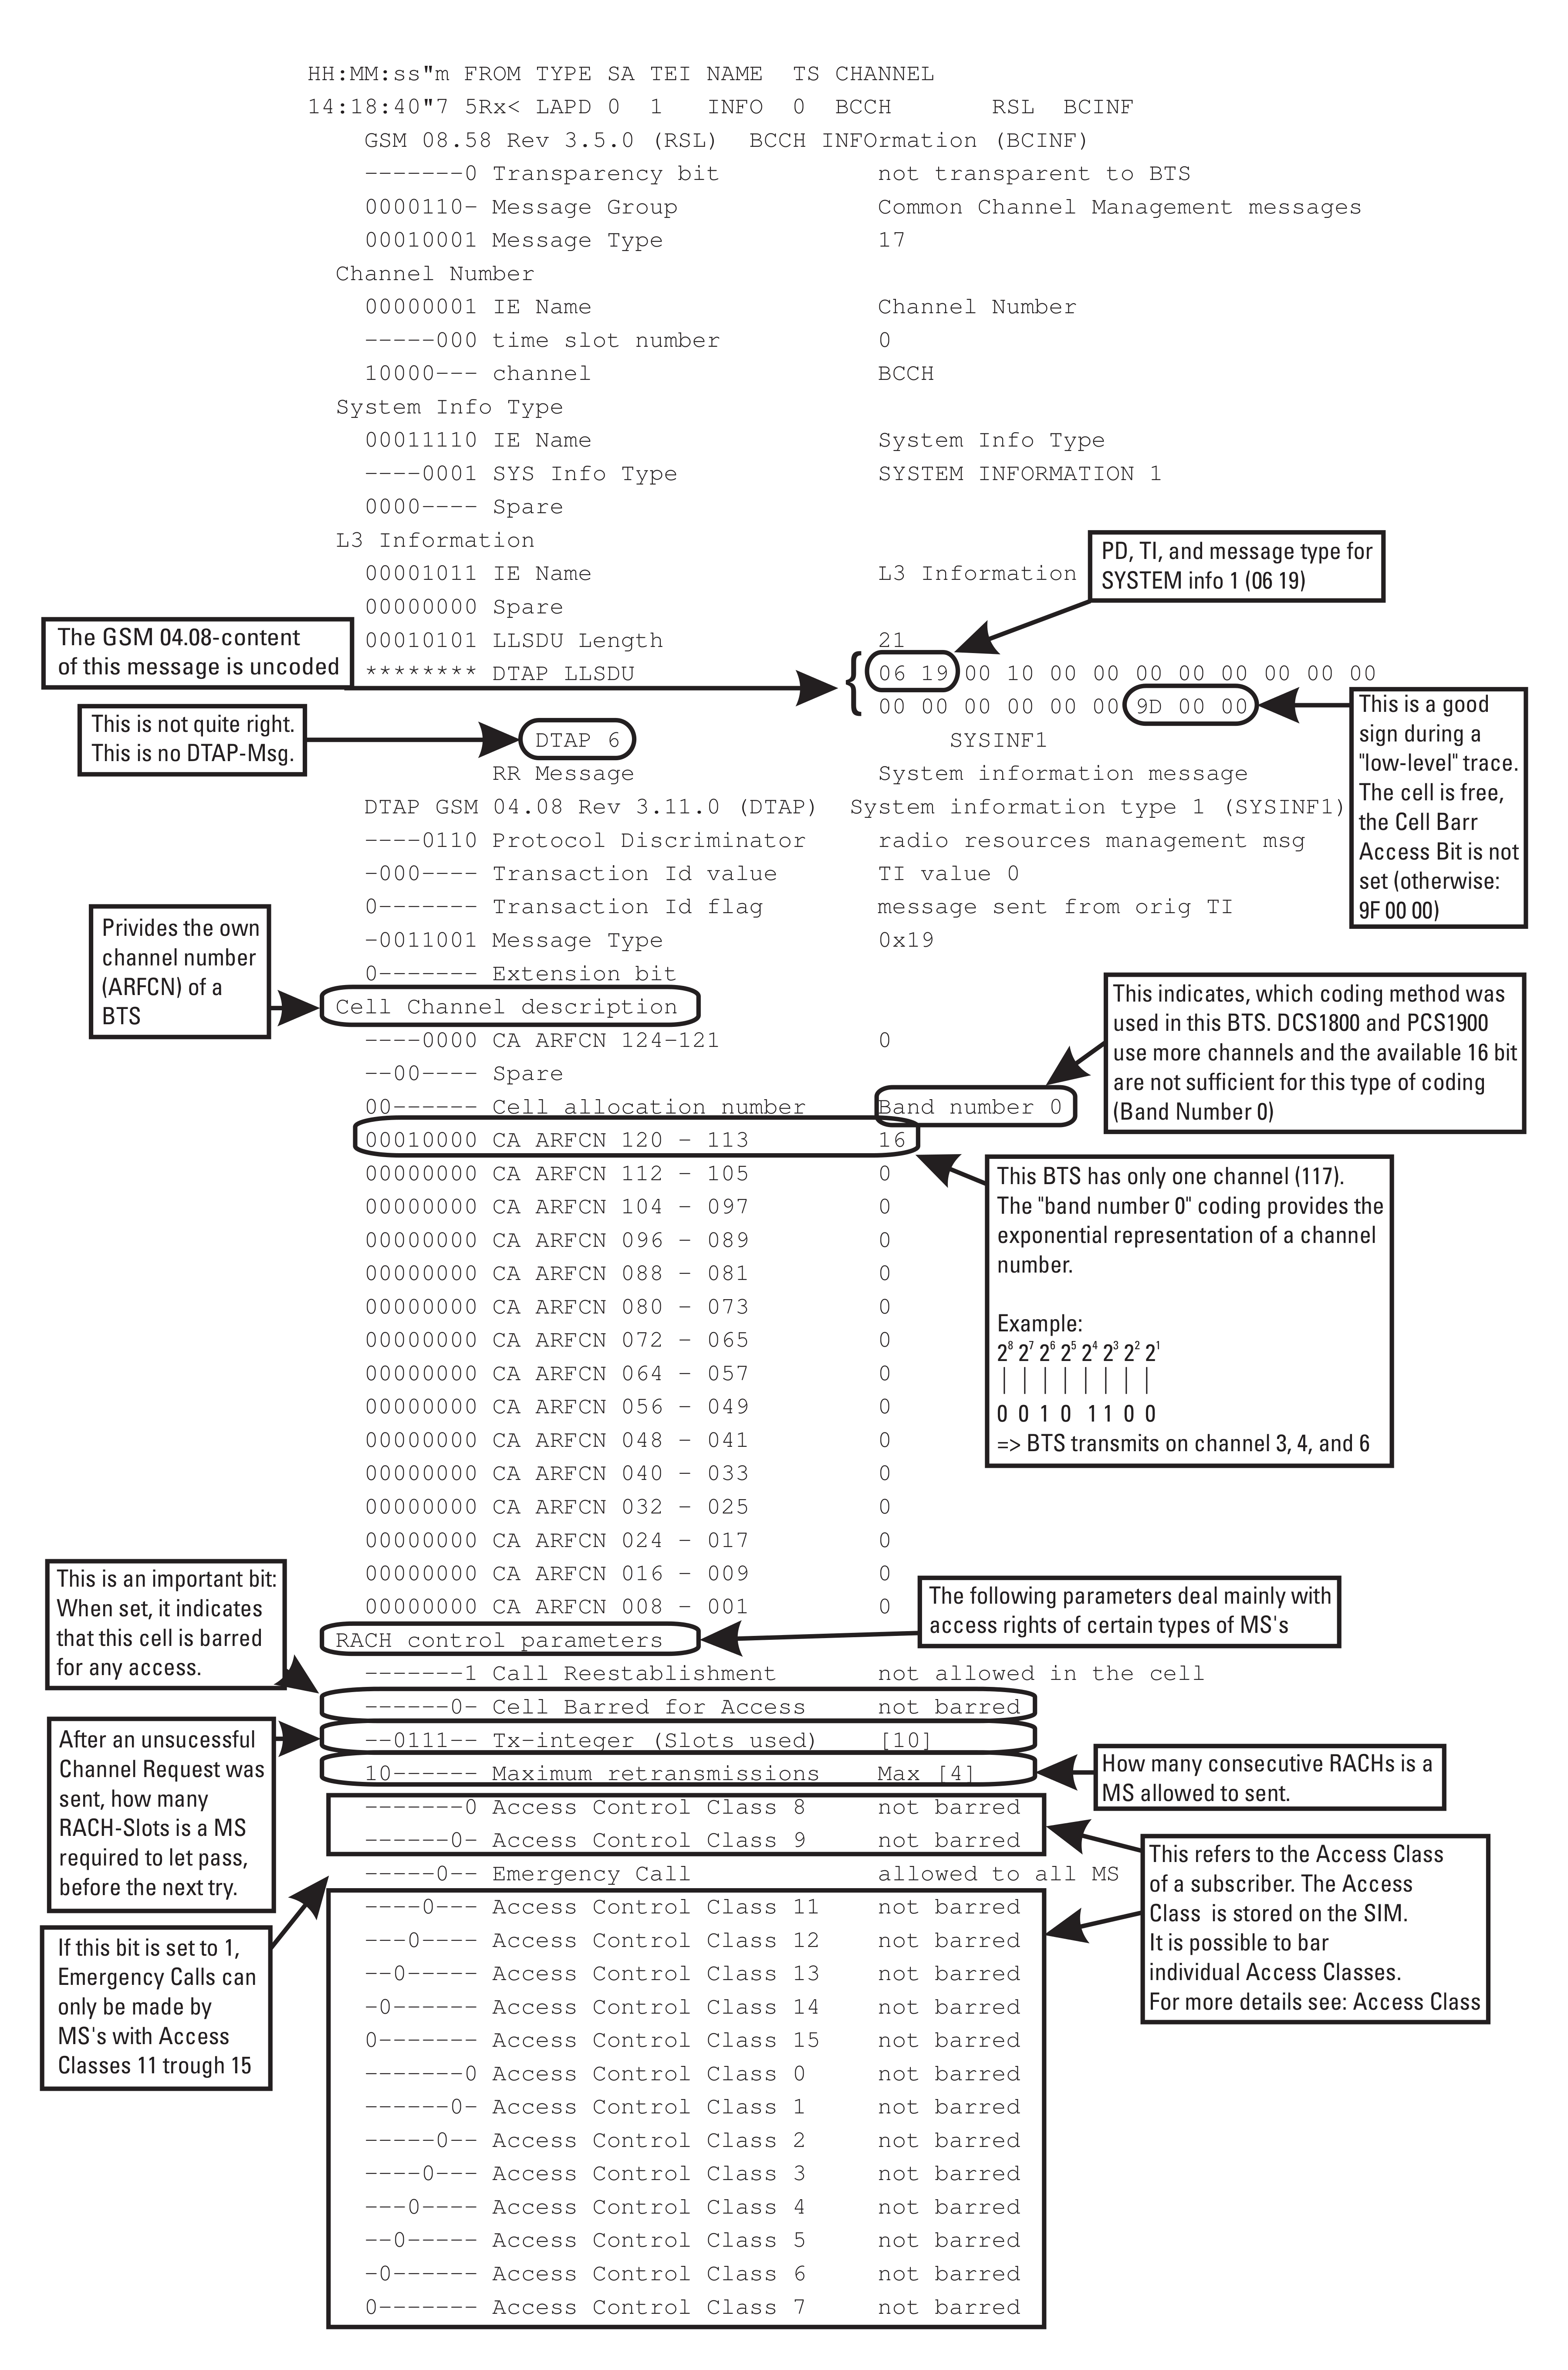
\includegraphics[width=.9\textwidth]{../Images/sysinfo1}
\caption{System Information 1 Message}
\end{figure}
\begin{figure}
\centering
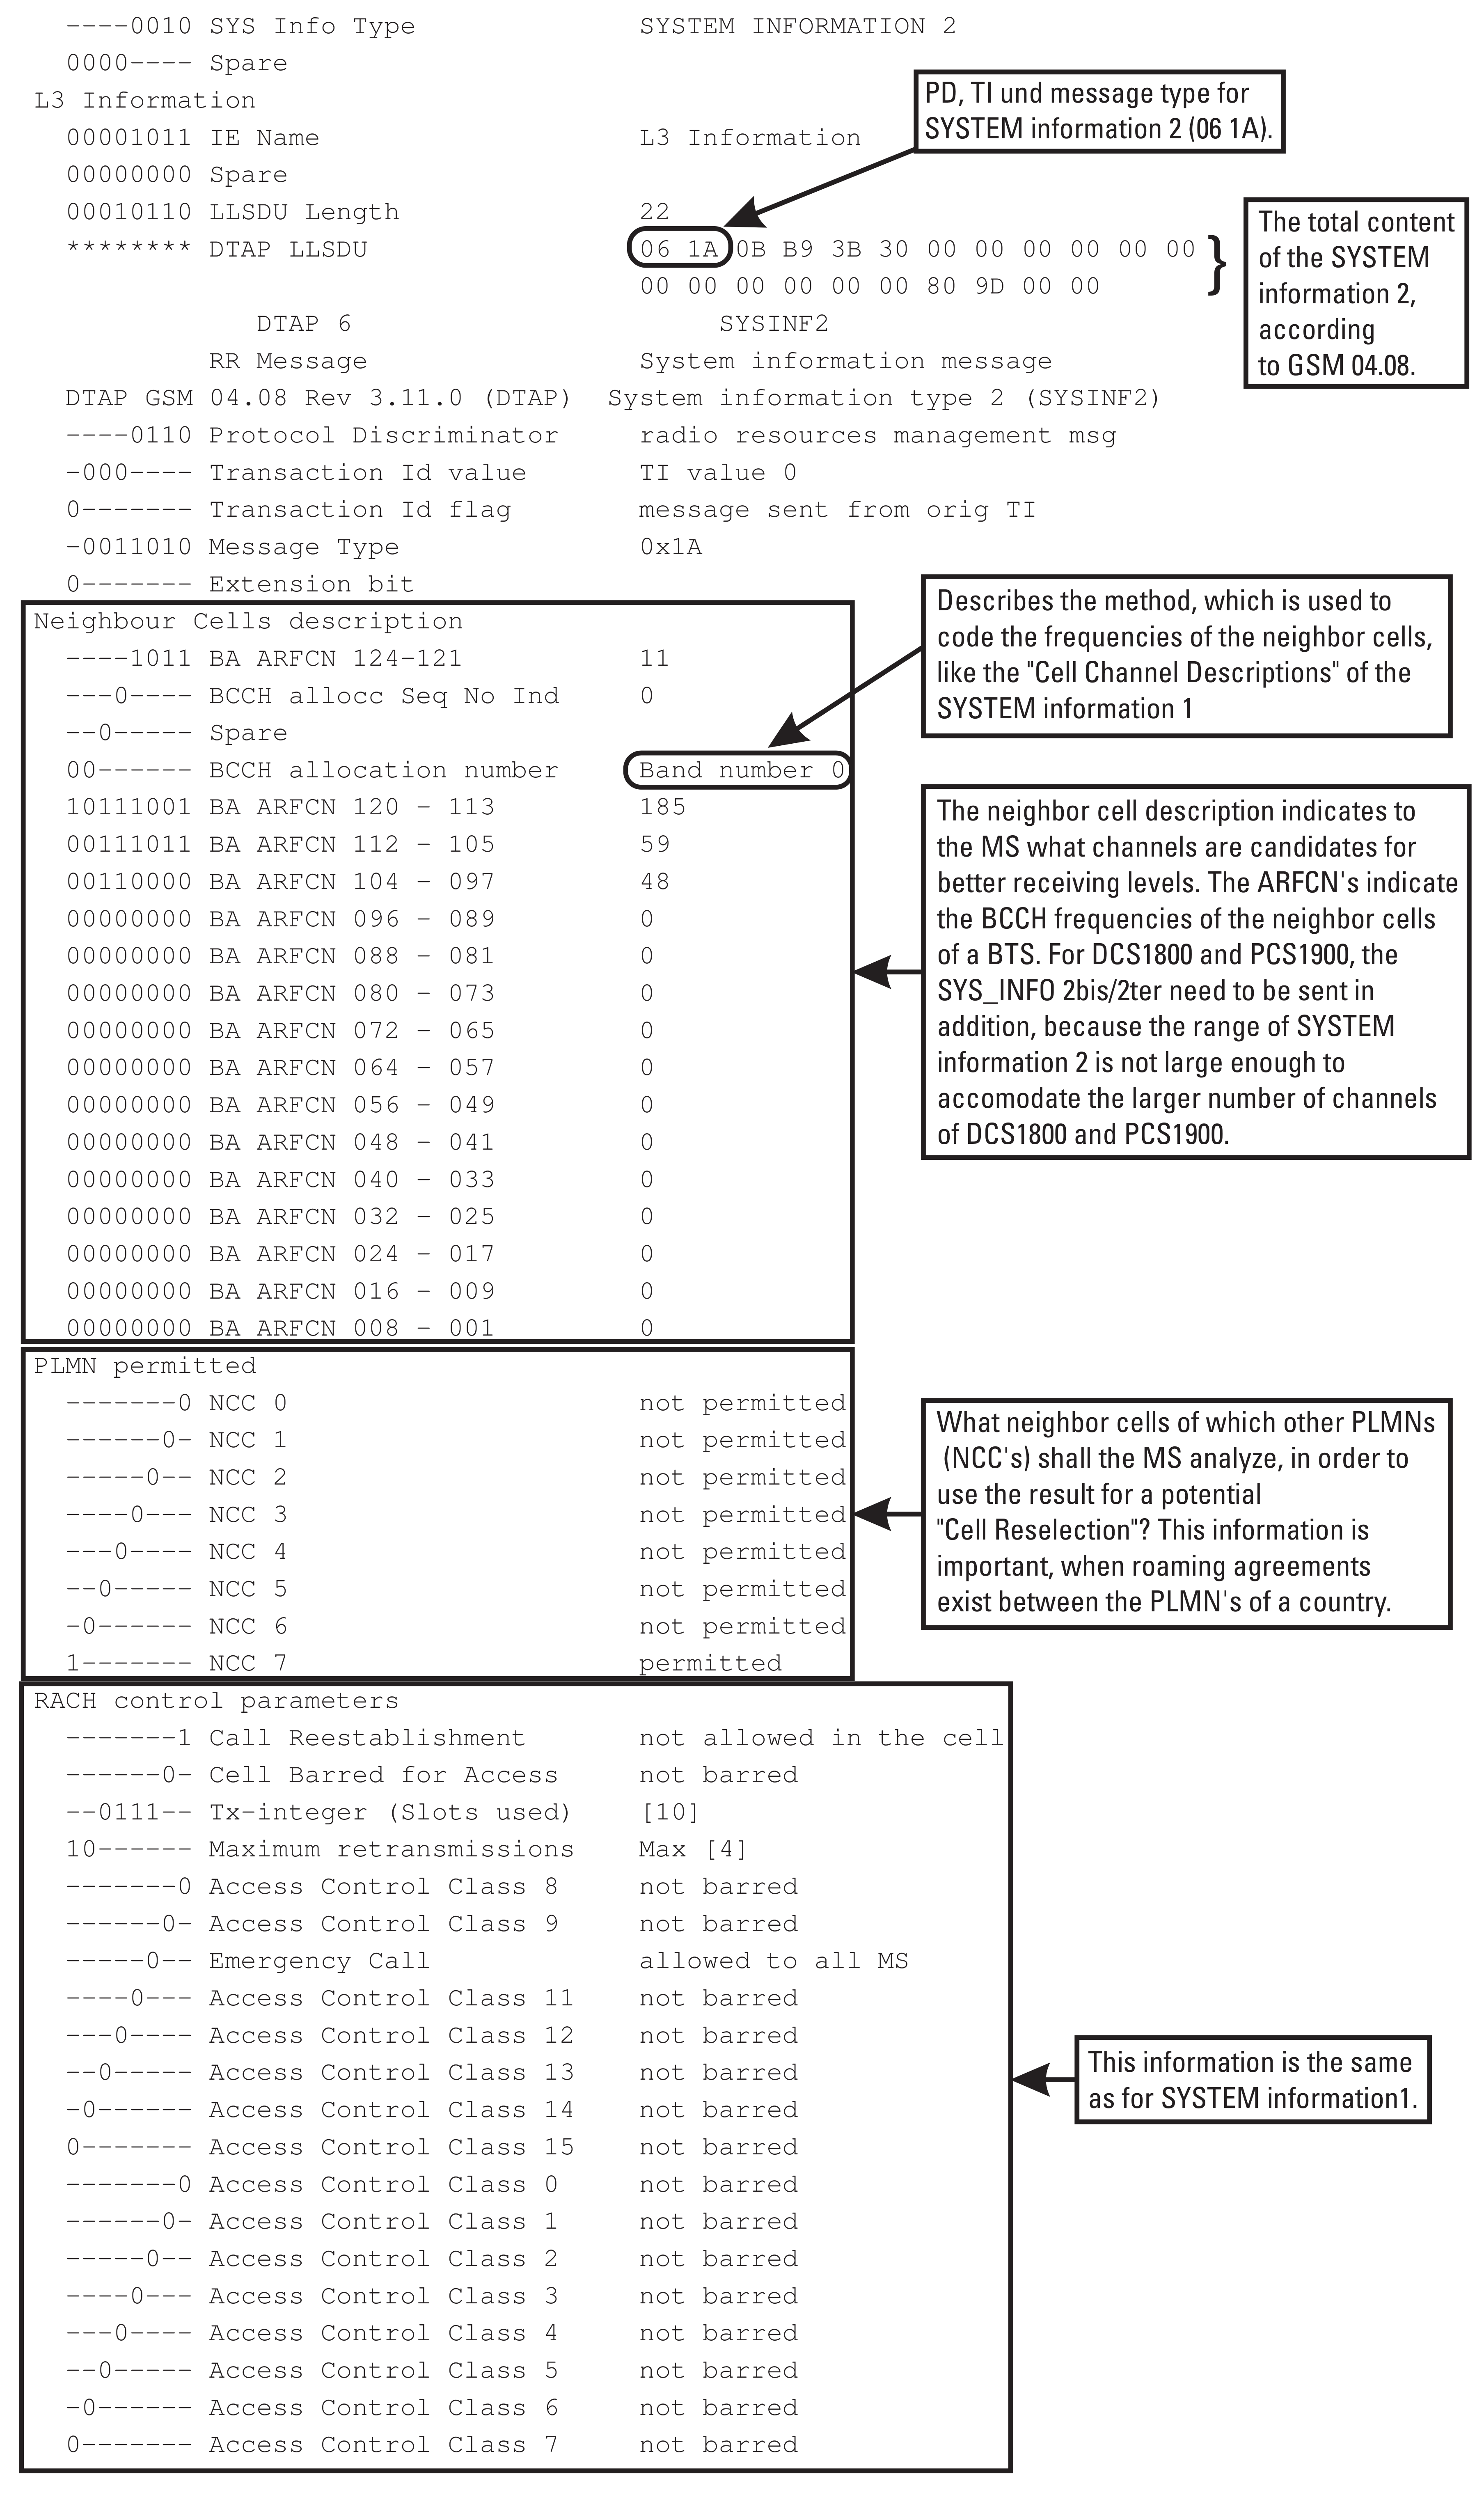
\includegraphics[width=.9\textwidth]{../Images/sysinfo2}
\caption{System Information 2 Message}
\end{figure}
\begin{figure}
\centering
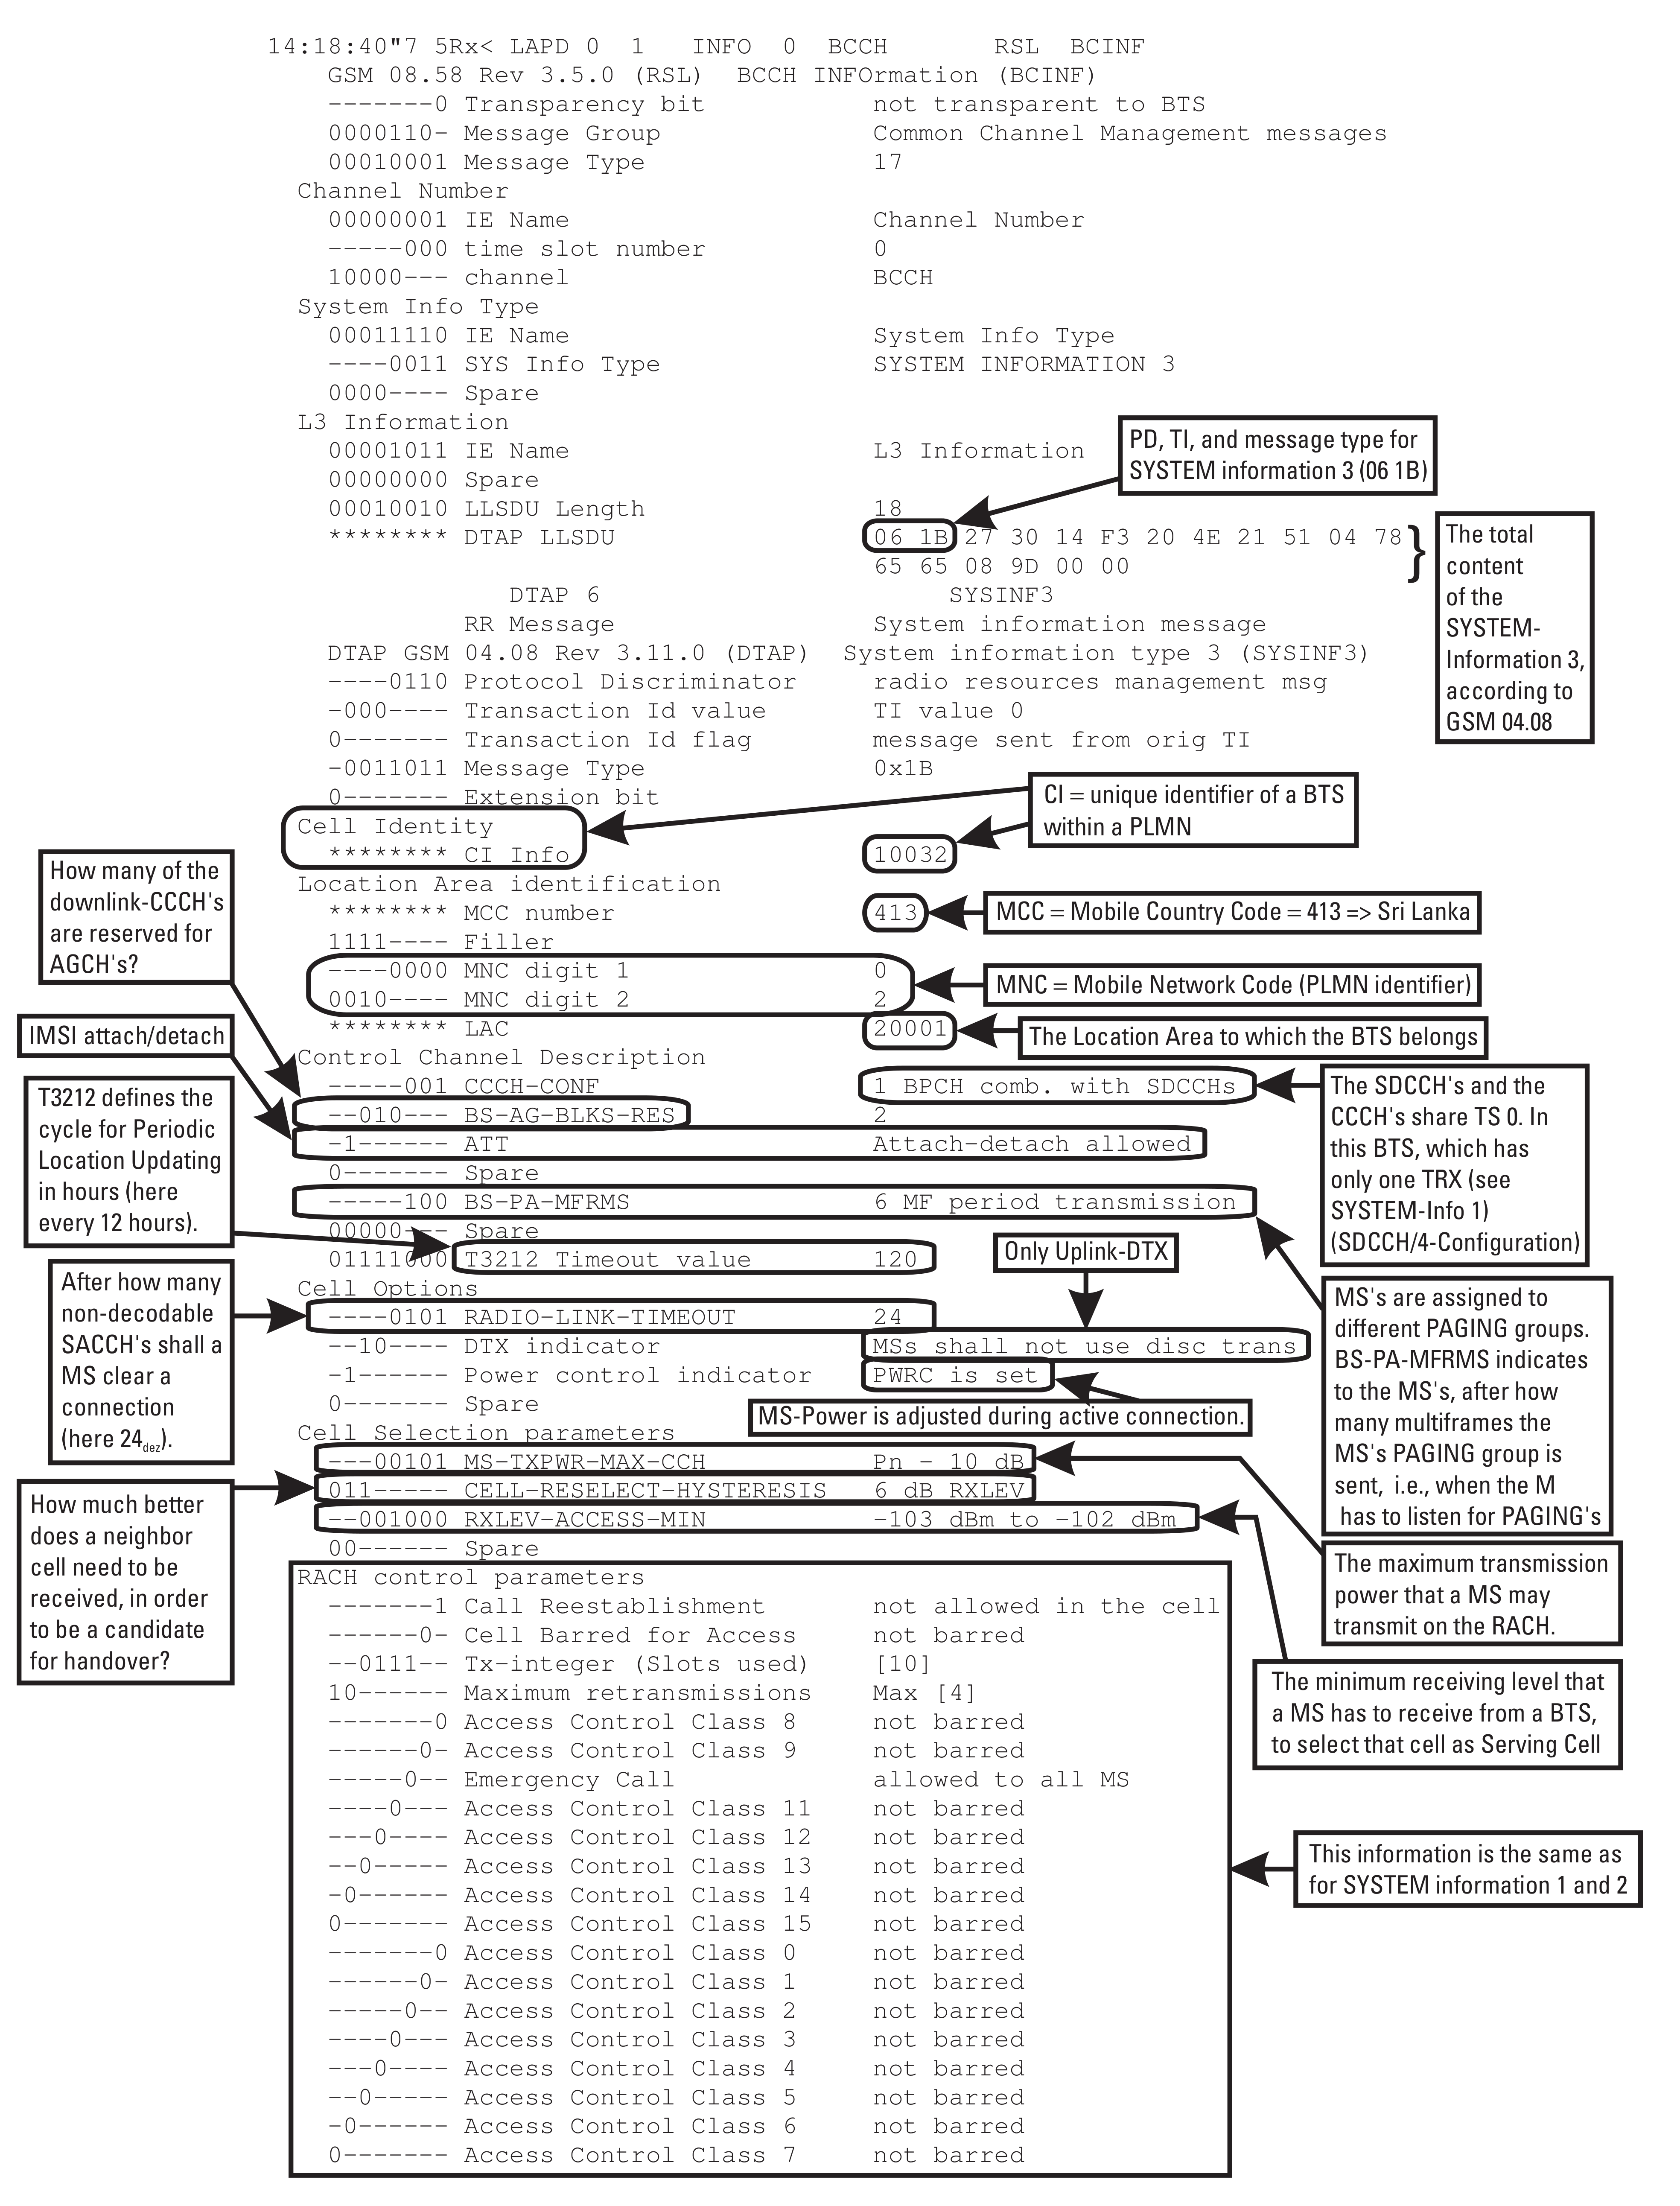
\includegraphics[width=.9\textwidth]{../Images/sysinfo3}
\caption{System Information 3 Message}
\end{figure}
\begin{figure}
\centering
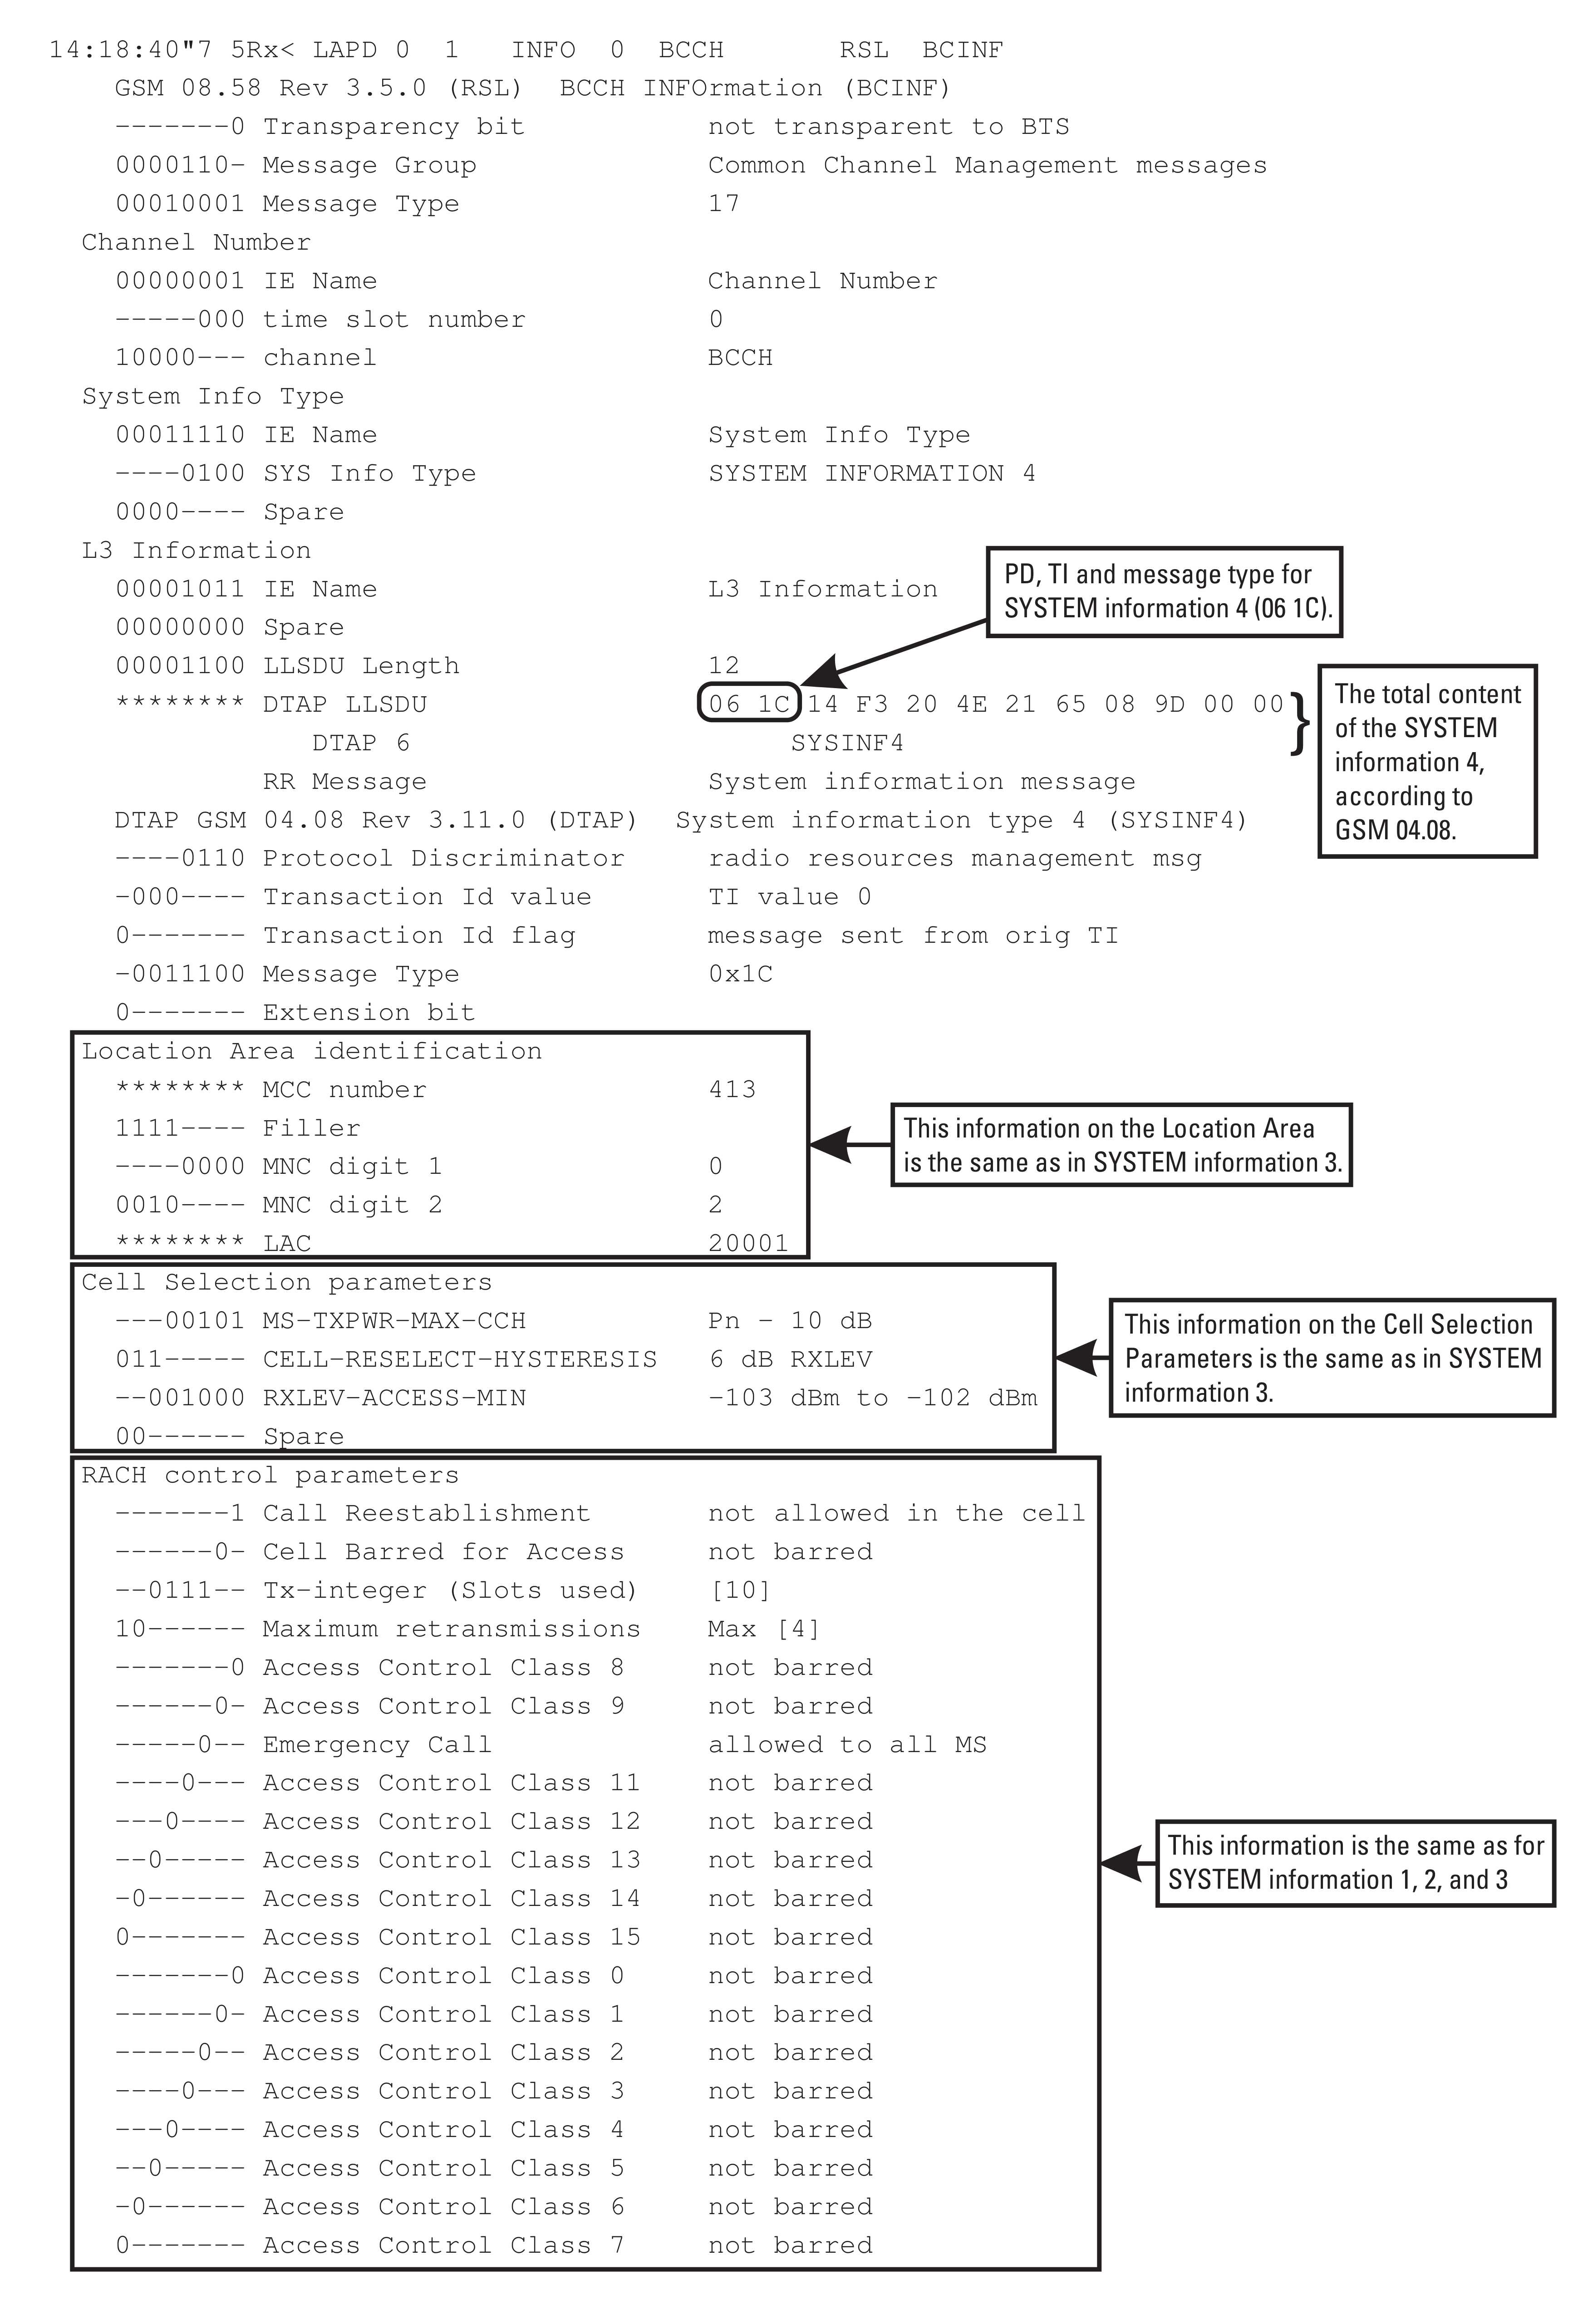
\includegraphics[width=.9\textwidth]{../Images/sysinfo4}
\caption{System Information 4 Message}
\end{figure}
\chapter{Evaluation Data}
\section{IMSI Catcher Configurations}
\section{ICDS Scans}